The centralized server architecture represents a most principal component in the hybrid edge-server person Re-ID system, serving as the computational backbone for resource-intensive operations that exceed the capabilities of edge devices. While the CPU-based edge devices handle distributed object detection and initial preprocessing, the centralized server leverages its GPU computing resources to perform sophisticated model inference tasks, including feature extraction and gender classification. Additionally, the server manages vector database operations for identity storage and retrieval, coordinates multi-consumer message processing from Kafka streams, and maintains the overall system state for cross-camera identity matching, as illustrated in Figure \ref{fig:centralized_server_overview}. This centralized microservice-based approach enables the system to achieve optimal resource utilization by offloading computationally demanding tasks from resource-constrained edge devices to a dedicated server environment equipped with specialized hardware acceleration. The server's architecture is designed to handle concurrent processing of multiple video streams while maintaining real-time performance requirements essential for practical surveillance applications.

\newpage
\begin{figure}[!htbp]
    \centering
    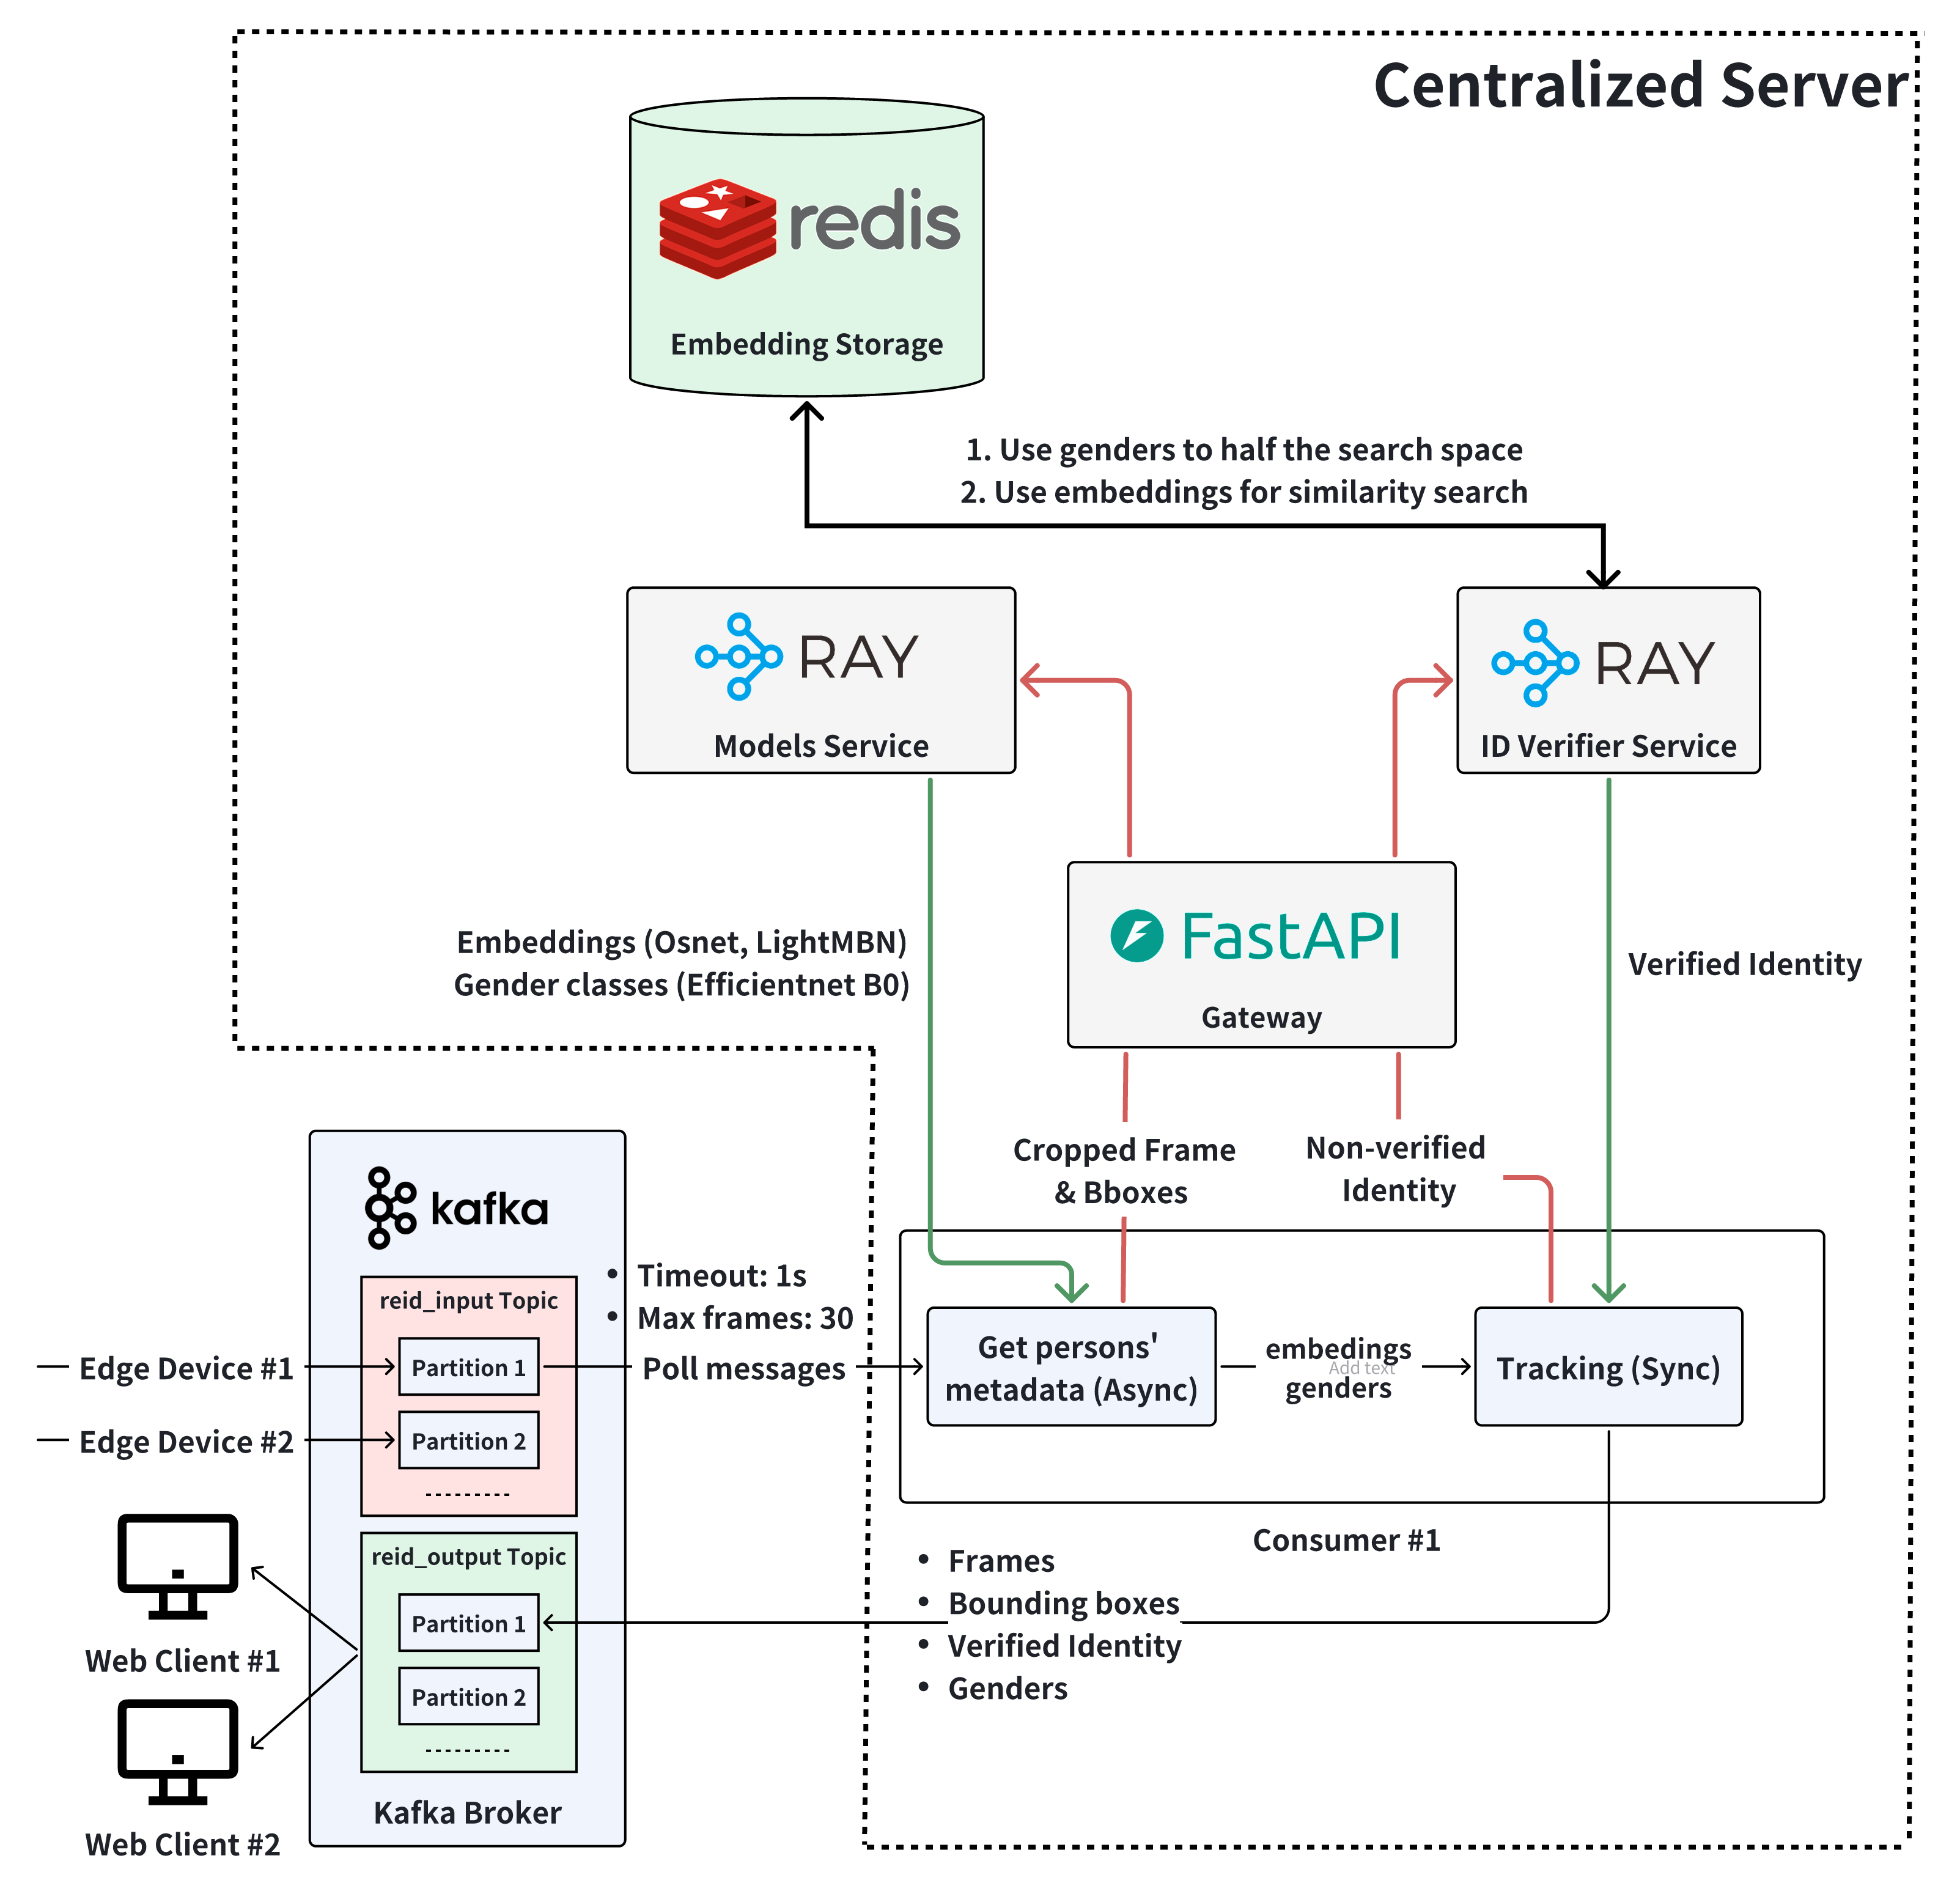
\includegraphics[width=1.1\textwidth]{Figure/centralized_overview.png}
    \caption{Centralized server architecture. The server is equipped with a decent GPU and CPU, and it is responsible for performing sophisticated model inference tasks, vector database operations, and multi-consumer message processing.}
    \label{fig:centralized_server_overview}
\end{figure}

\subsection{System Data Flow and Processing Pipeline}

The centralized server architecture orchestrates a complex data flow that transforms raw video streams into actionable identity verification results through multiple interconnected services. As depicted in Figure \ref{fig:centralized_server_overview}, the processing pipeline begins when edge devices capture and preprocess video frames, transmitting video frames, cropped person detections, and bounding box coordinates through Kafka message queues to the centralized server.

Each partition of the Kafka topics corresponds to a specific camera feed, and each consumer group is responsible for processing messages from a single partition, ensuring that message ordering is preserved—a critical requirement for the tracking module of the Re-ID system. As illustrated in Figure \ref{fig:centralized_server_overview}, Consumer \#1 represents the data processing pipeline that serves as a template for additional consumers. Each consumer operates within an event loop that fetches batched messages (maximum 30 messages) from its assigned Kafka topic partition every 1 second. This batched processing approach significantly reduces computational overhead compared to continuous message fetching, while maintaining near real-time processing capabilities essential for surveillance applications.

After receiving the batch of messages, the system processes each message (frame) to get the person's metadata through a structured pipeline:

\begin{enumerate}
   \item For each frame containing cropped person detections and bounding box coordinates, the system extracts person regions and computes two essential properties (referred to as person metadata):
   \begin{itemize}
       \item \textbf{Embedding vector}: A numerical feature representation of the person region used for similarity searches in the vector database to determine whether the person already exists in the system.
       \item \textbf{Gender classification}: The predicted gender of the person (male or female), enabling gender-based search space partitioning that reduces computational complexity by approximately 50\% by querying only relevant gender subsets during similarity matching operations.
   \end{itemize}
   \item The processing goal is to obtain complete results for all frames in the batch before proceeding to tracking and identity matching operations.
\end{enumerate}

The first processing step does not require maintaining frame order, as the primary objective is achieving accurate and efficient results that can be sorted by timestamp before performing tracking and identity matching. This independence from sequential processing makes asynchronous processing an optimal approach for the initial metadata extraction phase, allowing parallel computation of embeddings and gender classifications across multiple frames simultaneously to maximize throughput and minimize processing latency.


The \textbf{FastAPI Gateway} acts as the central coordination layer that orchestrates the processing pipeline between Kafka consumers and Ray Serve services. As depicted in Figure \ref{fig:centralized_server_overview}, when consumers poll batched messages (cropped frames and bounding boxes) from their assigned Kafka partitions, the processing follows a sequential workflow via the FastAPI Gateway. First, the \textbf{Get person's metadata (Async)} module sends all cropped frames in the batch to the \textbf{Models Service} for feature extraction (OSnet, LightMBN embeddings) and gender classification (EfficientNet B0). After all frames in the batch are processed, the results are sorted by their original timestamps to maintain temporal order before proceeding to the tracking phase.

The sorted embeddings and gender classifications are then forwarded to the customized \textbf{Tracking (Sync)} module, which iterates through each frame in correct timestamp order. The tracking module (ByteTrack or BOTSort) uses detection results and embeddings to perform association with previous tracklets, returning a list of person IDs for each frame. Crucially, only newly discovered IDs that do not exist in previous tracklets are considered "non-verified" and require database verification. This is because tracking algorithms can only maintain ID persistence in the short term and cannot determine whether a person actually existed in the system previously.

For these non-verified IDs, the tracking module requests the \textbf{ID Verifier Service} to query the Qdrant vector database using gender-based search space partitioning and embedding similarity search. Once verified identities are returned, the tracking module updates its tracklet data with the correct IDs, ensuring that subsequent frames do not require repeated database queries for the same person, as the tracking module only consults the ID verifier service when encountering new, unrecognized identities.

Processed results, including verified identities, gender classifications, bounding box coordinates, and confidence scores, are published back to Kafka output topics using the same partitioned structure. This bidirectional communication pattern enables multiple web clients to subscribe to specific camera feeds or system-wide notifications, supporting diverse use cases from real-time monitoring dashboards to alert systems and analytical reporting applications.

The architecture's microservice design ensures fault tolerance and independent scaling, where individual services can be replicated or upgraded without affecting the overall system operation, making it suitable for production deployment in enterprise surveillance environments.


\subsection{Models Service}

This section examines the implementation details of the \textbf{Models Service}, which performs feature extraction and gender classification on detected person regions. The service is built using Ray Serve, a scalable model serving library designed for building high-performance online inference APIs. Ray Serve provides several key features and performance optimizations specifically beneficial for serving PyTorch models, including dynamic request batching, multi-node and multi-GPU serving capabilities, and automatic load balancing across distributed computing resources.

\subsubsection{Ray Serve configuration}

The Ray Serve configuration defines the deployment parameters and resource allocation for the Models Service. This setup establishes a distributed serving environment optimized for concurrent model inference across multiple GPU-accelerated workers, as demonstrated in the following \texttt{config.yaml} file:

\begin{lstlisting}[language=yaml, caption=Ray Serve configuration file]
proxy_location: EveryNode
http_options:
    host: 0.0.0.0
    port: 8000
grpc_options:
    port: 9000
    grpc_servicer_functions: []
logging_config:
    encoding: TEXT
    log_level: INFO
    logs_dir: null
    enable_access_log: true
    additional_log_standard_attrs: []
applications:
    - name: thesis-model-serving
    route_prefix: /
    import_path: src.main.model_service
    runtime_env: {}
    deployments:
    - name: ModelService
        num_replicas: 4
        max_ongoing_requests: 32
        ray_actor_options:
        num_cpus: 2.0
        num_gpus: 0.25
\end{lstlisting}


\textbf{Network Configuration}: The service is configured to accept HTTP requests on port 8000 and gRPC requests on port 9000, with the proxy deployed on every node (\texttt{EveryNode}) to ensure load distribution and minimize network latency. The \texttt{0.0.0.0} host binding enables external access from edge devices and other system components.

\textbf{Resource Allocation Strategy}: The deployment specifies 4 replicas of the ModelService, each allocated 2.0 CPU cores and 0.25 GPU units. This fractional GPU allocation enables efficient GPU memory sharing, allowing multiple model inference processes to utilize the same GPU simultaneously. With 4 replicas sharing GPU resources, the system can achieve optimal GPU utilization while maintaining parallel processing capabilities.

The multiple replica strategy addresses a fundamental challenge in serving lightweight neural networks on GPU hardware. The deployed models are relatively compact: OSNet contains approximately 2 million parameters (~8MB model size), while EfficientNet B0 comprises around 5.3 million parameters (~21MB model size). These small model footprints significantly underutilize GPU computational resources when processed sequentially through traditional approaches such as iterative for-loops over bounding box detections.

Sequential processing of individual person regions results in GPU underutilization due to insufficient computational load per inference operation. Modern GPUs are designed for high-throughput parallel computation, but lightweight models cannot maximize usage of the available CUDA cores and tensor processing units. This mismatch leads to a processing bottleneck where the system becomes constrained by sequential execution rather than GPU computational capacity, resulting in suboptimal requests per second (RPS) performance that plateaus well below the hardware's theoretical maximum.

By deploying multiple replicas with fractional GPU allocation, the system transforms the inference pattern from sequential to parallel execution. Each replica can simultaneously process different batches of person detections, effectively multiplying the concurrent inference operations. This approach maximizes GPU utilization by ensuring that multiple inference operations are executed in parallel across different CUDA streams, saturating the GPU's computational resources and achieving significantly higher RPS throughput than single-replica deployments.

The 4-replica configuration with 0.25 GPU allocation per replica ensures that the total GPU memory and computational resources are fully utilized while preventing resource contention. This design enables the system to handle concurrent inference requests from multiple camera feeds efficiently, transforming the GPU from an underutilized resource in sequential processing to a fully optimized parallel processing engine capable of meeting real-time surveillance demands.

\textbf{Concurrency Management}: Each replica is configured to handle a maximum of 32 ongoing requests (\texttt{max\_ongoing\_requests: 32}), providing a total system capacity of 128 concurrent inference requests across all replicas. This configuration balances memory consumption with throughput requirements, preventing GPU memory overflow while maximizing processing efficiency.

\textbf{Request Batching Benefits}: The combination of multiple replicas and concurrent request handling enables Ray Serve's dynamic batching capabilities to automatically group incoming requests for batch inference. This batching mechanism significantly improves GPU utilization by processing multiple person regions simultaneously, reducing per-request inference time and increasing overall system throughput.

\textbf{Fault Tolerance and Scaling}: The multi-replica deployment provides inherent fault tolerance, where individual replica failures do not compromise system availability. Additionally, the configuration supports horizontal scaling by adjusting the \texttt{num\_replicas} parameter based on workload demands, enabling dynamic resource allocation in response to varying inference loads from multiple camera feeds.

This configuration strikes an optimal balance between resource utilization, processing latency, and system reliability, ensuring that the \textbf{Models Service} can efficiently handle the computational demands of real-time person Re-ID applications across distributed edge-server architectures.

\subsubsection{Feature extraction}

The feature extraction component represents the core computational module of the Models Service, responsible for transforming raw person detection images into numerical feature representations suitable for similarity matching and identity verification. The implementation leverages two state-of-the-art person Re-ID models—OSNet and LightMBN—each optimized for different aspects of feature extraction performance and accuracy.

\begin{enumerate}
    \item \textbf{Cold start problem}:\\
    The cold start problem in deep learning model serving refers to the initial latency penalty incurred during the first inference request, caused by GPU memory allocation, CUDA kernel compilation, and model weight loading operations. To mitigate this issue, the Models Service implements a comprehensive warmup strategy during initialization through the \texttt{\_warmup()} method. This approach creates dummy input tensors with the exact dimensions required by each model: \texttt{torch.randn(1, 3, 256, 128)} for OSNet and LightMBN models, and \texttt{torch.randn(1, 3, 224, 224)} for the EfficientNet gender classification model. By executing forward passes with these dummy inputs during service startup, the system pre-allocates GPU memory, compiles necessary CUDA kernels, and initializes all computational graphs, ensuring that subsequent real inference requests experience minimal latency without the overhead of first-time GPU operations.
    
    \item \textbf{Image preprocessing}:\\
    Initially, image bytes from the API are in raw bytes format, so we need to decode them to \texttt{Image.PIL} format using \texttt{BytesIO} and the function \texttt{Image.open()}. The preprocessing pipeline ensures consistent input format by converting non-RGB images to RGB mode using \texttt{Image.convert("RGB")}, which is essential for maintaining color channel consistency across different input image formats.

    The system implements two distinct preprocessing pipelines optimized for different model requirements:
    
    \textbf{Embedding models (OSNet and LightMBN)}: Images are resized to 256×128 pixels to match the input dimensions expected by person Re-ID models, which are specifically designed for person-centric aspect ratios. The preprocessing applies ImageNet normalization with mean=[0.485, 0.456, 0.406] and std=[0.229, 0.224, 0.225] to ensure compatibility with pre-trained model weights.
    
    \textbf{Classification model (EfficientNet)}: Images are resized to 224×224 pixels, the standard input size for EfficientNet architectures, and normalized using the same ImageNet statistics to maintain consistency with pre-training data distribution.
    
    Both pipelines convert images to PyTorch tensors using \texttt{transforms.ToTensor()}, which automatically scales pixel values from [0, 255] to [0, 1] range and reorders dimensions from HWC (Height-Width-Channel) to CHW (Channel-Height-Width) format required by PyTorch models.
    
    \item \textbf{OSNet model}:\\
    The OSNet (Omni-Scale Network) model serves as the primary feature extraction backbone, initialized with \texttt{osnet\_x1\_0} architecture containing 1000 output classes for comprehensive feature representation. The model is loaded with pre-trained weights (\texttt{pretrained=True}) and configured with softmax loss for optimal person Re-ID performance. OSNet's distinctive architecture employs omni-scale convolutions that capture multi-scale features simultaneously, making it particularly effective for person Re-ID tasks where scale variations are common due to different camera distances and viewing angles. The model processes 256×128 input images and outputs feature vectors that capture discriminative person characteristics essential for cross-camera identity matching.
    
    \item \textbf{LightMBN model}:\\
    The LightMBN (Lightweight Multi-Branch Network) model provides an alternative feature extraction approach optimized for computational efficiency while maintaining competitive accuracy. Initialized with 512 feature dimensions and configured without activation mapping (\texttt{activation\_map=False}) for streamlined inference, LightMBN outputs features in shape [batch\_size, 512, 7], where the 7 components represent different spatial regions of the person image. The system applies average pooling across these 7 components using \\ \texttt{features.mean(dim=2)} to produce a consolidated 512-dimensional feature vector, effectively combining multi-region information into a single representative embedding suitable for similarity calculations and database storage.
    
    \item \textbf{API gateway implementation}:\\
    The Models Service exposes three distinct API endpoints, each optimized for different usage patterns and performance requirements:
    
    \begin{itemize}
        \item \textbf{Single image API} (\texttt{/embedding}): Designed for low-latency applications requiring immediate response, this endpoint processes individual images through the \texttt{extract\_features\_single} method. It prioritizes response time over throughput, making it suitable for interactive applications or real-time processing scenarios where each request must be handled independently without waiting for batch formation.
        
        \item \textbf{Dynamic batching API} (\texttt{/embedding/batch}): Leverages Ray Serve's automatic batching capabilities with \texttt{@serve.batch} decorator configured for maximum batch size of 32 images and 10ms timeout \\(\texttt{batch\_wait\_timeout\_s=0.01}). This endpoint automatically groups concurrent requests into batches, optimizing GPU utilization by processing multiple images simultaneously while maintaining acceptable latency. The dynamic batching approach balances throughput optimization with responsiveness, automatically adapting to varying request loads.
        
        \item \textbf{True batching API} (\texttt{/embedding/true-batch}): Processes multiple images submitted as a single request through the \texttt{List[UploadFile]} parameter, enabling clients to explicitly control batch composition. For PyTorch models, the system utilizes matrix calculations to stack individual image tensors into a single batch tensor using\\ \texttt{torch.cat(processed\_images, dim=0)}, then performs inference on the entire batch vector simultaneously. This approach maximizes computational efficiency by leveraging GPU's parallel processing capabilities for matrix operations, significantly reducing inference time compared to sequential processing. The batched inference returns results for all images in a single forward pass, eliminating the overhead of individual request processing and maximizing GPU computational throughput for scenarios where multiple images are available simultaneously, such as processing video frame sequences or bulk image analysis tasks.
    \end{itemize}
    
    Each API endpoint returns structured responses containing feature vectors, dimensional information, and processing metadata, enabling clients to select the most appropriate processing mode based on their specific latency and throughput requirements.
\end{enumerate}

\subsubsection{Gender classification}

The gender classification component serves as an optimization module within the Models Service, designed to reduce computational complexity in identity verification by enabling gender-based search space partitioning. This approach leverages the biological distinction between male and female individuals to partition the vector database, effectively reducing the search space by approximately 50\% during similarity matching operations when implemented. The implementation utilizes a custom-trained EfficientNet B0 model specifically optimized for person gender classification tasks, as detailed in Section \ref{sec:classification_experiments}.

\textbf{Model Architecture and Configuration}: The gender classification model is built upon the EfficientNet B0 architecture, a compound scaling method that uniformly scales network width, depth, and resolution with a set of fixed scaling coefficients. The model is initialized through the \texttt{GenderClassificationModel} class and configured to process 224×224 pixel RGB images, matching the standard input dimensions for EfficientNet architectures. The model outputs binary classification logits representing male and female categories, with softmax activation applied to generate probability distributions for confidence scoring.

\textbf{Custom Training Approach}: Unlike the pre-trained person Re-ID models (OSNet and LightMBN), the gender classification model represents a custom-trained solution developed specifically for this surveillance system. The training methodology, dataset composition, and performance evaluation are comprehensively documented in Section \ref{sec:classification_experiments}, where detailed experimental results demonstrate the model's effectiveness in distinguishing gender characteristics from person detection crops under various lighting conditions, viewing angles, and image qualities typical in surveillance environments.

\textbf{Preprocessing Pipeline}: The gender classification preprocessing follows the same ImageNet normalization standards as the embedding models but with distinct dimensional requirements. Input images are resized to 224×224 pixels to match EfficientNet's expected input dimensions, converted to RGB format for color consistency, and normalized using mean=[0.485, 0.456, 0.406] and std=[0.229, 0.224, 0.225]. This preprocessing ensures optimal compatibility with the model's learned feature representations while maintaining consistency with standard computer vision practices.

\textbf{API Implementation}: The gender classification functionality is exposed through the \texttt{/gender/classify} endpoint, which processes individual images and returns structured predictions including the predicted gender label, confidence score, and probability distributions for both male and female categories. The API implementation follows the same preprocessing pipeline as other model endpoints, utilizing the \texttt{preprocess\_single} method with "efficientnet" model specification to ensure appropriate image transformations.

The inference process applies softmax activation to the model's logits using \texttt{F.softmax(logits, dim=1)} to generate normalized probability distributions, followed by \texttt{torch.argmax} to determine the predicted class. The system maps numerical predictions to human-readable labels using a predefined mapping where class 0 corresponds to "male" and class 1 corresponds to "female". Additionally, the API returns confidence scores extracted from the maximum probability value, enabling downstream systems to implement confidence-based filtering or uncertainty quantification.

\textbf{Search Space Optimization}: The primary motivation for gender classification lies in its ability to significantly reduce computational overhead during identity verification queries. By classifying detected persons into gender categories, the system can partition the vector database and limit similarity searches to gender-specific subsets. This optimization reduces the average number of embedding comparisons by approximately 50\%, directly translating to faster query response times and improved system scalability. The gender-based partitioning strategy is particularly effective in surveillance scenarios where gender distribution is typically balanced, ensuring that both partitions contribute meaningfully to search space reduction without creating significant load imbalances.

\subsection{Embedding Storage}

\subsubsection{Qdrant configuration}

\subsubsection{Retrieval approach}

\subsection{ID Verifier Service}

\subsection{Consumers}